\documentclass{acm_proc_article-sp}

\usepackage{graphicx}
\usepackage{float}
\usepackage{hyperref}

\begin{document}

\title{Parallel Video Processing}
\subtitle{[Parallel Programming Final Project Report]
\titlenote{}}

\numberofauthors{3} 
\author{
% 1st. author
\alignauthor
Po-Han Chen\titlenote{}\\
       \affaddr{National Chiao Tung University}\\
       \email{j.lin013@gmail.com}
% 2nd. author
\alignauthor
Cheng Sun\titlenote{}\\
       \affaddr{National Chiao Tung University}\\
       \email{s2821d3721@gmail.com}
% 3rd. author
\alignauthor 
Yu-Wen Pwu\titlenote{}\\
       \affaddr{National Chiao Tung University}\\
       \email{yuwen41200@gmail.com}
}

\maketitle
\begin{abstract}
Video processing typically requires immense amounts of computational resources. Devices supporting up to 4K resolution are currently hitting the market by storm. A greater demand for computation has thus arisen. Therefore, we set out to explore ways to boost the efficiency of video processing through a series of experiments. These experiments were conducted with a wide assortment of tools(or APIs) on multiple platforms. We've managed to achieve what we consider maximum possible speedups on our test platforms. 
\end{abstract}

\section{Introduction}
Initially, we were interested in whether parallelizing simple image processing tasks could deliver any speedup. A number of image processing tasks rely on matrix multiplications which take only constant number of computations per pixel. This gives O(N) complexity and likely higher memory access frequencies. \\
Seeing these computations are reasonably simple, we suspected that compilers might optimize programs to an extent where speeding up with parallelization might not be possible. To test this out, we designed and conducted 2 experiments, Lightup and Lightup2. The former does simple arimetic calculations on each pixel, while the latter multiplies each pixel by \(1.125^{(x+y)/128}\). From these experiments, we concluded that increasing the amount of computations per thread does raise speedups and that different platforms(or OSes) along with different optimization options are not the reasons for the subtle speedups in Lightup. \\
Our research into parallel video processing branched out from here. We decided to have a closer look at the feasibility of using FPGAs to speedup video processing. We consider FPGAs a suitable choice for heterogeneous computing because FPGAs are essentially massively parallel processors. Fully customized hardware designs can lead to maximized optimization. In the end, we were able to obtain nearly 1000x speedup on a 1920*1080 dataset. This was also 100x faster than other approaches. \\
Unsatisfied with Lightup experiments, we've found and tested a tool called pmbw - Parallel Memory Bandwidth Benchmark / Measurement \cite{pmbw}. It's a tool written in assembly that tests important memory characteristics including maximum bandwidth on our test platforms. After examining the test results from pmbw, we believed a speedup of up to 3.2x should be attainable. \\
We then turned our attention to real-world problems. We decided to use White balance as our video processing application. The White balance algorithm \cite{gray_world} we used takes O(N) time and was simple enough for us to experiment with. We used 5 different parallelization approaches: Pthread\_TDM, OpenMP\_TDM, CUDA, CUDA\_TDM and TaskParallel (We will detail these approaches in later contexts). While CUDA still delivers poor results due to frequent global memory accesses, Pthread and OpenMP managed to yield 3x speedups on the main test platform and 2x speedups on the secondary test platform. Both numbers were consistent with the test results from pmbw. We concluded that certain hardware characteristics do pose an "invisible ceiling" especially in I/O bound applications and CUDA on consumer-grade GPUs might not be suitable for this type of applications.

\section{Proposed Solutions: Lightup series (CPU/GPU)}
\subsection{Lightup}
For each pixel, \([R', G', B'] = [R, G, B * 2 + 5] \) \\
Then normalize the RGB values back to [0, 255]. \\
This would increase the overall blue contrast.
\subsection{Lightup}
For each pixel, \([R', G', B'] = [R, G, B * 1.125^{(x + y) / 128}]\) \\
Then normalize the RGB values back to [0, 255]. \\
The blue channels would become mostly 0's (ie. image becomes yellowish) except for the bottom-right corner. \\
\\
* We will discuss our parallelization methods with White balance altogether in later contexts.

\section{Proposed Solutions: Lightup2.5 (FPGA)}
\subsection{Lightup2.5}
For each pixel, \([R', G', B'] = [R, G, B] * 1.125^{1024}\)
\subsection{Considerations}
The performance of the circuit is highly dependent on the quality of the circuit design and the available resources on the FPGA development board. Although some EDA (electronic design automation) tools, like Xilinx SDAccel, support high-level synthesis that can convert OpenCL C/C++ codes into schematics, these techniques are not mature enough, and may lead to poor performance.
\subsection{Implementation}
We employ RTL (register-transfer level) design by the Verilog HDL (hardware description language), and we use the Xillybus IP core \cite{fpga_ref} for data transmission over the PCIe interface. Our targeted board is Xilinx Virtex-5 ML506 Evaluation Platform. We use C++ for software design. The host programs run on a 64-bit Linux.
\begin{figure}[H]
  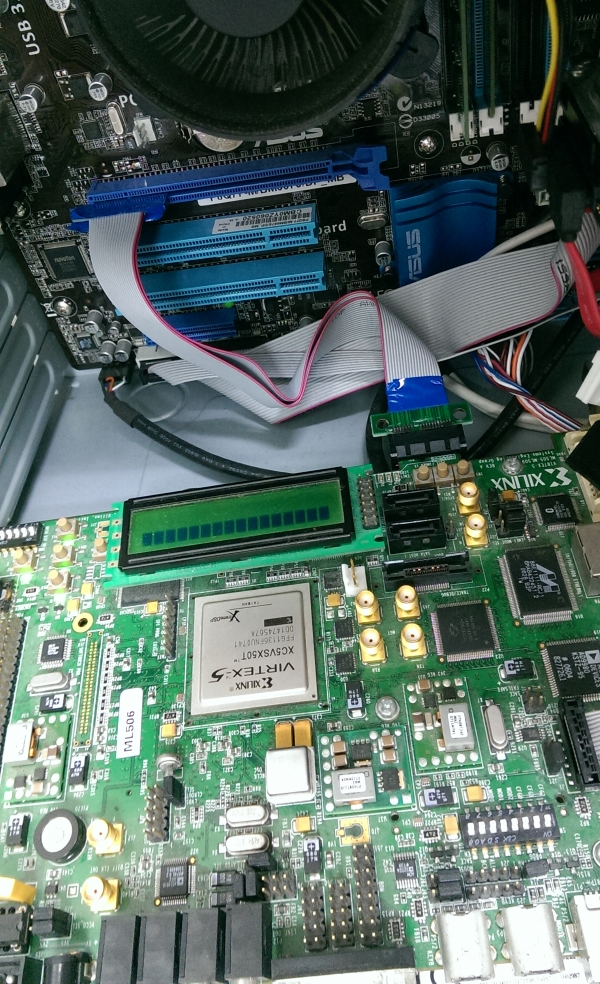
\includegraphics[width=\linewidth,natwidth=600,natheight=984]{fpga_connect.jpg}
  \label{fig:fpga_connect}
\end{figure}
\subsection{Computation Platform}
The PC-end (host) is on the left side, whereas the FPGA-end (device) is on the right side.
\begin{figure}[H]
  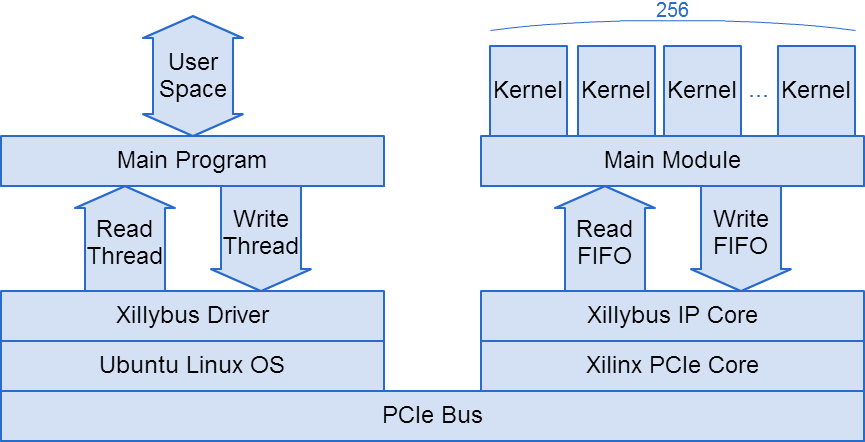
\includegraphics[width=\linewidth,natwidth=865,natheight=442]{fpga_block.png}
  \label{fig:fpga_block}
\end{figure}
\subsubsection{Data Interface}
To hosts, the device looks just like a file. So we can use low-level (POSIX) file I/O functions to read/write data from/to the device, i.e. the FPGA board.
\subsubsection{Multithreading on Software}
For best performance, we have 2 threads implemented on the host program. The first is used to send data, the other is used to receive data.
\subsection{Kernel Instantiation}
We use a \textit{generate block} to instantiate 256 kernel modules, namely, 256 simultaneously running threads. Each kernel module calculates a single color value, so the FPGA can calculate at most 256 values at the same time.
\subsubsection {Finite State Machine}
4 states: IDLE\_STATE, RECV\_STATE, EXEC\_STATE, and SEND\_STATE. After the program starts, the circuit goes to the second state. The second state waits and receives 256 color values, until then, it goes to the third state. The third state processes the 256 received values in parallel, then it goes to the last state. The last state waits and sends 256 new values back, and goes to the first state again.

\section{Proposed Solutions: White balance}
\subsection{Block diagram}
Input and Calculate are parallelizable.
\begin{figure}[H]
  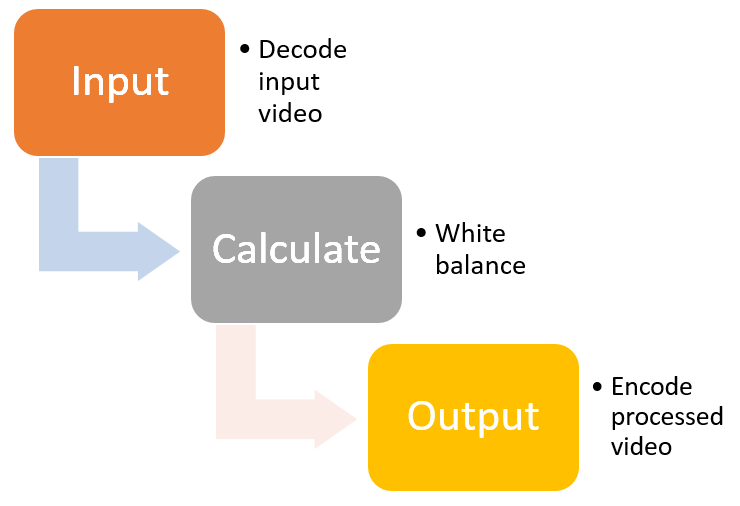
\includegraphics[width=\linewidth,natwidth=740,natheight=506]{block_diagram.png}
  \label{fig:block_diagram}
\end{figure}
\subsection{Algorithm}
\begin{enumerate}
  \item Calculate the averages of Red, Green and Blue values, as denoted by (AvgR, AvgG, AvgB)
  \item Using Green as reference, for each pixel, \\
    \(Red_{new} = Red * AvgG / AvgR\) \\
    \(Blue_{new} = Blue * AvgG / AvgB\)
  \item If \(Red,Blue_{new} > 255\) Then \(Red,Blue_{new} = 255\)
\end{enumerate}
\subsection{Initialization}
With scalability in mind and to prevent memory exhaustion, we divide the input video into chunks with each containing no more than 500 frames. \\
\begin{figure}[H]
  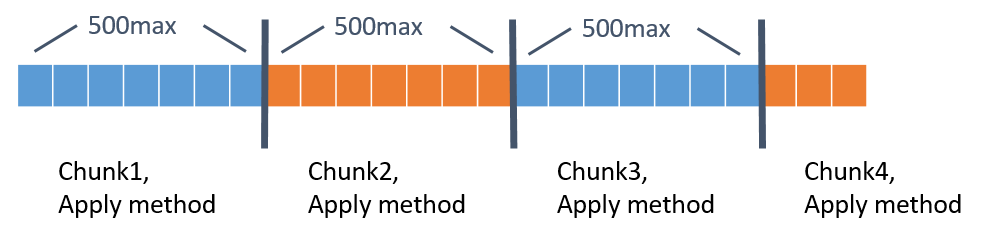
\includegraphics[width=\linewidth,natwidth=986,natheight=233]{chunks.png}
  \label{fig:chunks}
\end{figure}
\subsection{Parallel method1: Pthread}
We process one frame at a time. We let each thread process a portion of columns.
\begin{figure}[H]
  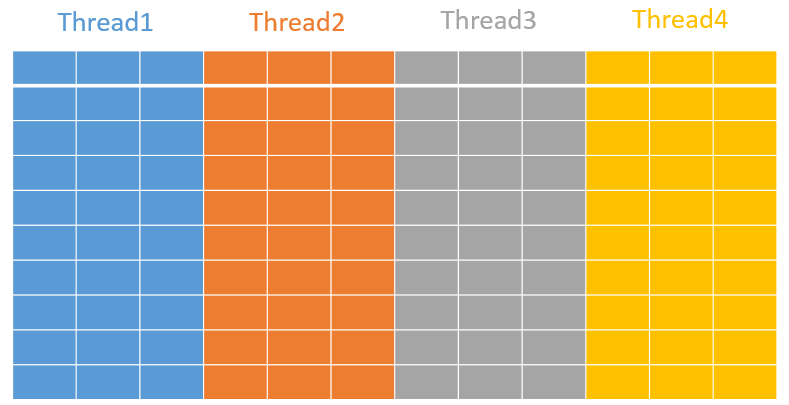
\includegraphics[width=\linewidth,natwidth=789,natheight=405]{Pthread.png}
  \label{fig:TDM}
\end{figure}
\subsection{Parallel method2: Pthread\_TDM}
Utilizing C++11 threading libraries, we divide the input video by time. Each thread is assigned a collection of video frames as indicated by the following figure. \\
\begin{figure}[H]
  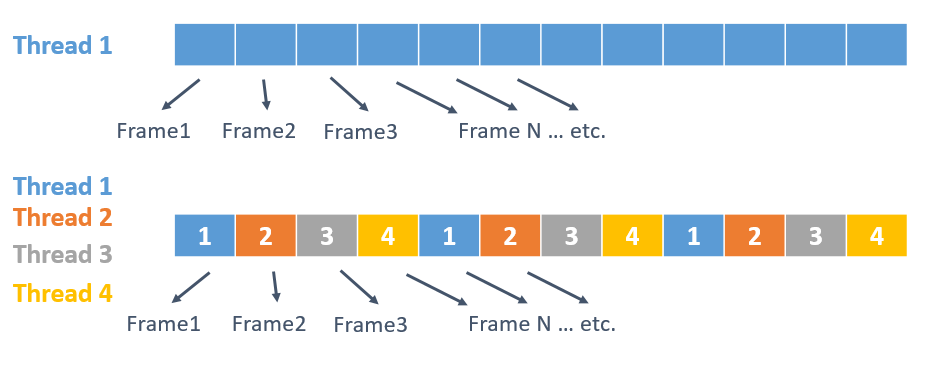
\includegraphics[width=\linewidth,natwidth=934,natheight=370]{TDM.png}
  \label{fig:TDM}
\end{figure}
\subsection{Parallel method3: OpenMP\_TDM}
We also divide the input video by time, but with OpenMP as the API.
\subsection{Parallel method4: CUDA}
We process one frame in each iteration(as in memcpy operation pairs). Each thread processes one pixel.
\begin{figure}[H]
  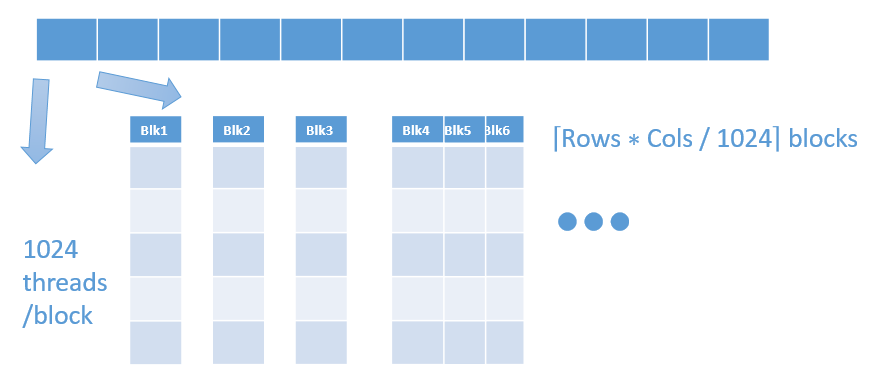
\includegraphics[width=\linewidth,natwidth=874,natheight=376]{CUDA.png}
  \label{fig:CUDA}
\end{figure}
\subsection{Parallel method5: CUDA\_TDM}
Very similar to previous approaches, we divide the input video by time where each thread block processes one frame.
\begin{figure}[H]
  
\includegraphics[width=\linewidth,natwidth=766,natheight=114]{CUDA_TDM.png}
  \label{fig:CUDA_TDM}
\end{figure}
\subsection{Parallel method6: Pthread\_with\_TaskParallel}
Extended from Pthread\_TDM, rather than waiting for Input and Calculate to finish, we create a separate thread specifically for output. 
\begin{figure}[H]
  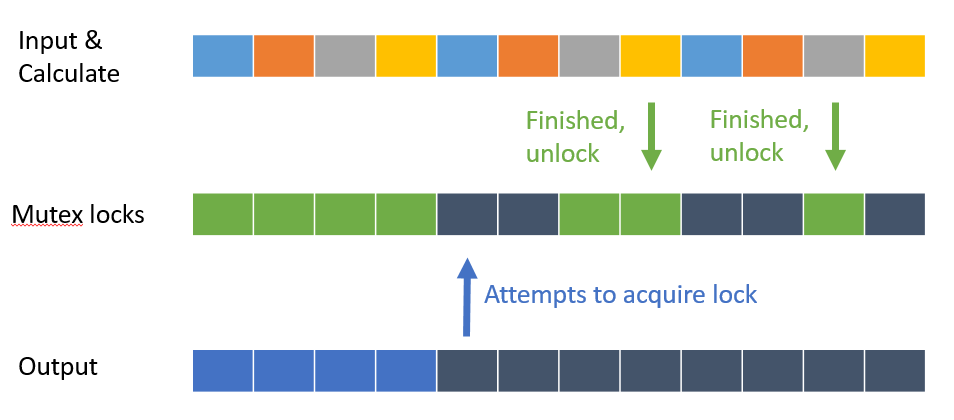
\includegraphics[width=\linewidth,natwidth=954,natheight=420]{Pthread_with_TaskParallel.png}
  \label{fig:Pthread_with_TaskParallel}
\end{figure}


\section{Experimental Methodology}
\subsection{Environment specifications}
APIs: OpenCV 2.4.11, OpenCV 3.0 \\
\begin{table}[H]
\centering
\begin{tabular}{|l|l|l|l|} \hline
OS&CPU&RAM&Compiler\\ \hline
Windows 10 & i7-3770(4C8T) & 16GB & VS12, gcc 5.2.0 \\ \hline
Ubuntu 14.04 & i5-4200H(2C4T) & 8GB & gcc 4.8.4 \\ \hline
OSX El Capitan & i5-4260U(2C4T) & 8GB & gcc 5.2.0\\ \hline
Ubuntu 15.10 & 2 vCores & 2GB & gcc 5.2.0 \\ \hline
\end{tabular}
\end{table}
GPU (on i7 PC): GeForce GTX 670, CUDA v7.5, CUDA Capability 3.0. \\
\\
FPGA Board: Xilinx Virtex-5 ML506 Evaluation Platform. \\
FPGA Host PC: Ubuntu 14.04, i5-3570(4C4T), 8GB, gcc 5.3.0.
\subsection{Input datasets}
\subsubsection{Lightup \& Lightup2:}
 360*240 / 1280*720 / 1920*1080, 148 frames (MP4). \\
\subsubsection{Lightup2.5:}
 256*256 / 1920*1080*3 (Raw data). \\
\subsubsection{White balance:}
 1280*720, 1422Frames (MP4, AVI). \\

\subsection{Output}
\subsubsection{Lightup \& Lightup2:}
During visual inspection, the programs display the output video in realtime.
\subsubsection{Lightup2.5:}
Raw data (arrays) of sizes 256*256 / 1920*1080*3.
\subsubsection{White balance:}
If output is opted in (through C macro definition), the programs produce videos in the same resolution as input in AVI format. 

\section{Experimental Results}
\subsection{Lightup}
Slowdown when input is small. Tiny speedup even when input is large. Similar results across OpenCV 2.4, Ubuntu, OSX.
\begin{figure}[H]
  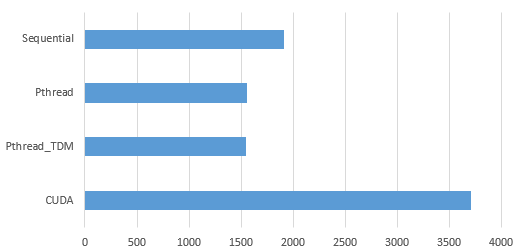
\includegraphics[width=\linewidth,natwidth=526,natheight=251]{lightup.png}
  \caption{Lightup (4 Threads, i7-3770, OpenCV3, VS12, Windows 10)}
  \label{fig:lightup}
\end{figure}
\begin{figure}[H]
  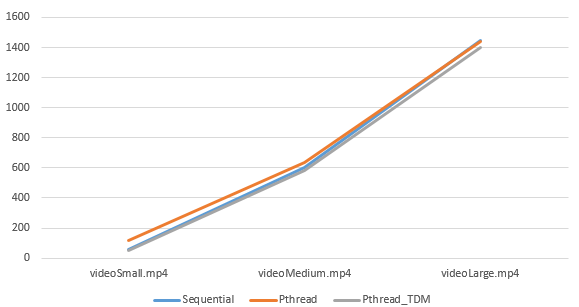
\includegraphics[width=\linewidth,natwidth=579,natheight=307]{lightup_sml.png}
  \caption{Lightup (4 Threads, i7-3770, OpenCV3, Cygwin-gcc 5.2.0, Windows 10)}
  \label{fig:lightup_sml}
\end{figure}
\begin{figure}[H]
  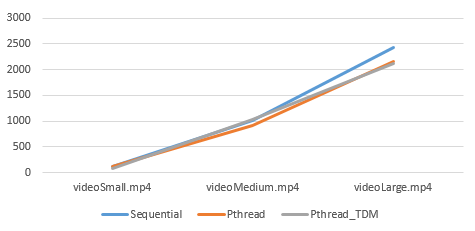
\includegraphics[width=\linewidth,natwidth=475,natheight=231]{lightup_osx.png}
  \caption{Lightup (4 Threads, i5-4260U, OpenCV3, gcc 5.2.0, OSX El Capitan)}
  \label{fig:lightup_osx}
\end{figure}
\subsection{Lightup2}
The results are clearly better than Lightup. Pthread\_TDM seems to be better than Pthread.
\begin{figure}[H]
  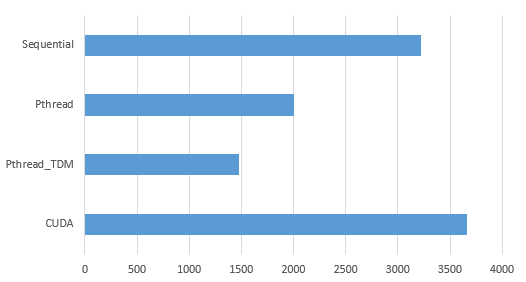
\includegraphics[width=\linewidth,natwidth=526,natheight=282]{lightup2.png}
  \caption{Lightup2 (4 Threads, i7-3770, OpenCV3, VS12, Windows 10)}
  \label{fig:lightup2}
\end{figure}
\begin{figure}[H]
  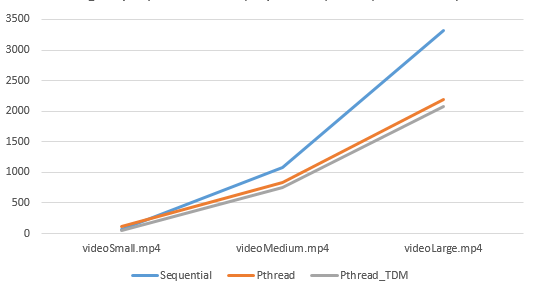
\includegraphics[width=\linewidth,natwidth=535,natheight=285]{lightup2_sml.png}
  \caption{Lightup2 (4 Threads, i7-3770, OpenCV3, Cygwin-gcc 5.2.0, Windows 10)}
  \label{fig:lightup2_sml}
\end{figure}
\begin{figure}[H]
  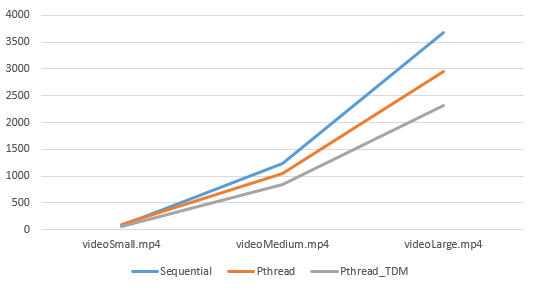
\includegraphics[width=\linewidth,natwidth=536,natheight=290]{lightup2_ubuntu.png}
  \caption{Lightup2 (4 Threads, i5-4200H, OpenCV3, gcc 4.8.4, Ubuntu 14.04)}
  \label{fig:lightup2_ubuntu}
\end{figure}

\subsection{Lightup2.5 (FPGA)}
Whopping speedups. FPGA is more than 100x faster than all other APIs.
\begin{table}[H]
\centering
\caption{Lightup2.5 Runtimes}
\begin{tabular}{|l|l|l|l|l|} \hline
Size&Sequential&OpenMP&CUDA&FPGA\\ \hline
Small & 179.096ms & 67.667ms & 891.333ms & \textbf{0.534ms} \\ \hline
Large & 15873.200ms & 4678.667ms & 1799.333ms & \textbf{16.104ms} \\ \hline
\end{tabular}
\end{table}
\begin{table}[H]
\centering
\caption{Lightup2.5 Speedups}
\begin{tabular}{|l|l|l|l|l|} \hline
Size&Sequential&OpenMP&CUDA&FPGA\\ \hline
Small & 1.00x & 2.65x & 0.20x & \textbf{335.39x} \\ \hline
Large & 1.00x & 3.39x & 8.82x & \textbf{985.67x} \\ \hline
\end{tabular}
\end{table}
\begin{figure}[H]
  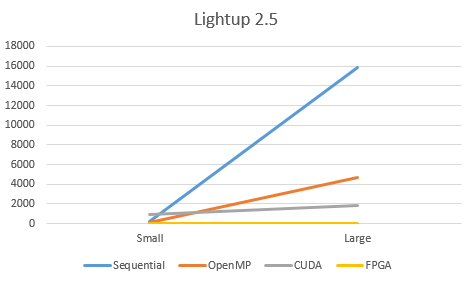
\includegraphics[width=\linewidth,natwidth=476,natheight=282]{lightup25_comparison.png}
  \label{fig:lightup2.5_comparison}
\end{figure}

\subsection{pmbw - Parallel Memory Bandwidth Benchmark / Measurement}
From the results below, we conclude that I/O should be parallelization-worthy (ie. speeding up is possible). Also, the upper bound looks to be around 3.2x (on the main test platform).
\begin{figure}[H]
  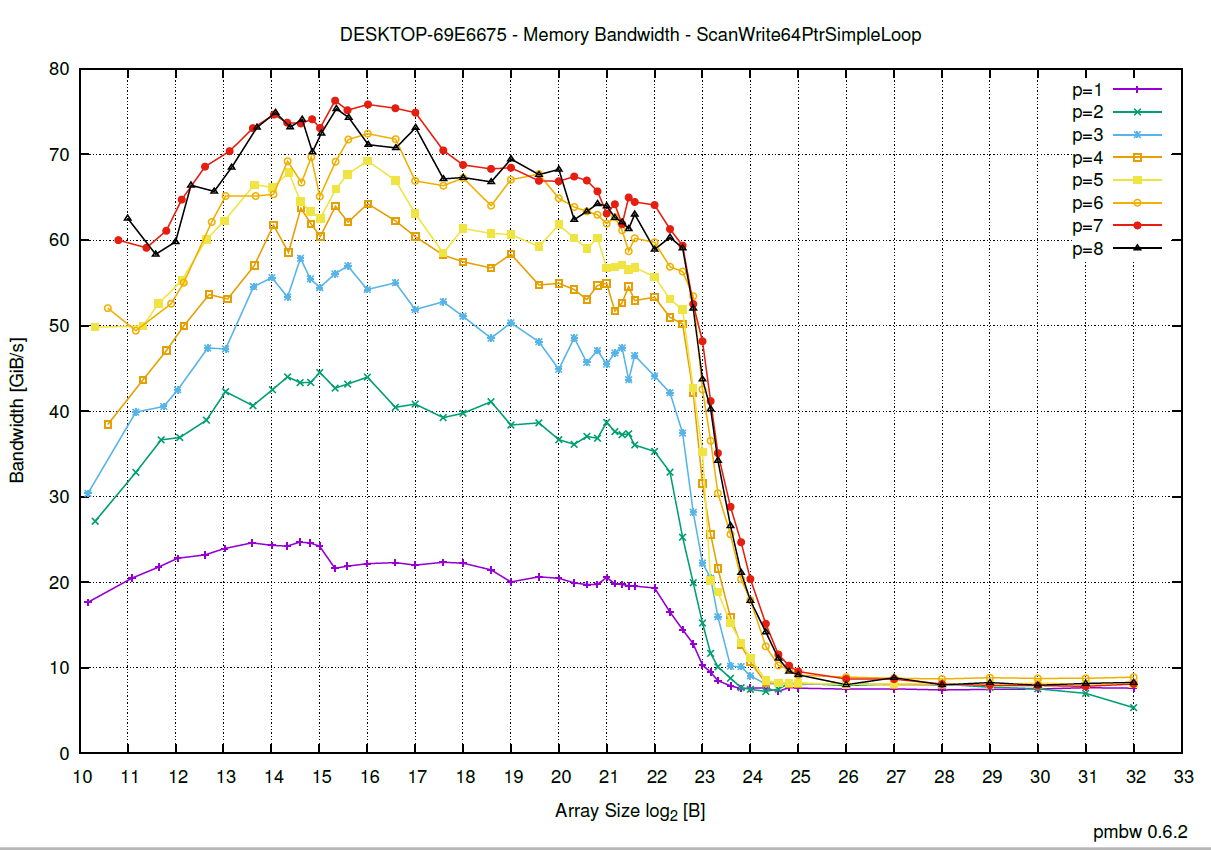
\includegraphics[width=\linewidth,natwidth=1211,natheight=850]{pmbw.png}
  \label{fig:pmbw}
\end{figure}

\subsection{White balance}
\begin{figure}[H]
  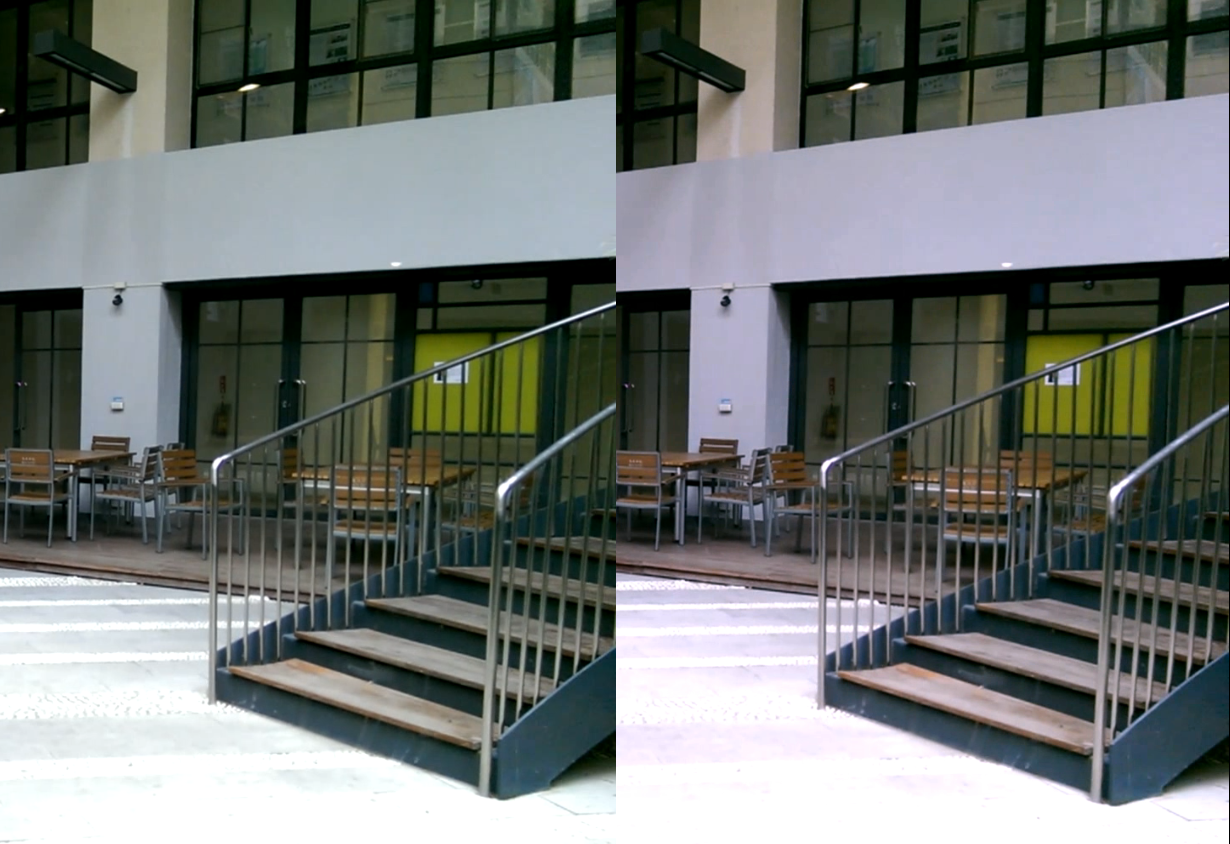
\includegraphics[width=\linewidth,natwidth=1230,natheight=844]{whitebalance_comparison.png}
  \caption{White balance Results: Before and After}
  \label{fig:whitebalance_comparison}
\end{figure}
\textbf{2 Threads}, i7-3770, VS12, Windows 10: \\
Pthread\_TDM: 1.69x speedup \\
OpenMP\_TDM: 1.77x speedup \\
CUDA: 0.80x slowdown \\
CUDA\_TDM: 0.41x slowdown
\begin{figure}[H]
  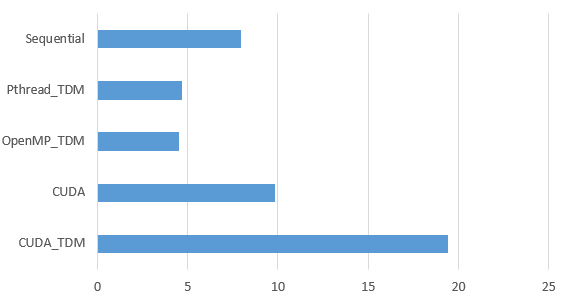
\includegraphics[width=\linewidth,natwidth=569,natheight=299]{white2.png}
  \caption{2 Threads, i7-3770, VS12, Windows 10}
  \label{fig:white2}
\end{figure}
\subsection{White balance and more threads}
We can see our approaches toward white balance do benefit from more threads.
The highest speedup we get is consistent with the results from pmbw.
\begin{table}[H]
\centering
\caption{White balance Speedups with more threads}
\begin{tabular}{|l|l|l|l|l|l|} \hline
Threads&1&2&4&6&8\\ \hline
Pthread\_TDM & 1.00x & 1.69x & 2.49x & 2.76x & 3.02x \\ \hline
OpenMP\_TDM & 1.00x & 1.77x & 2.76x & 2.92x & 3.00x \\ \hline
\end{tabular}
\end{table}
\begin{figure}[H]
  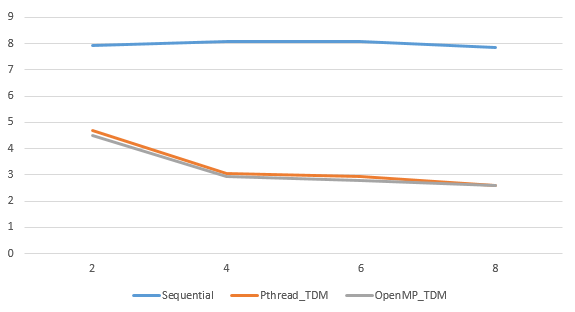
\includegraphics[width=\linewidth,natwidth=575,natheight=312]{white_morethreads.png}
  \caption{White Balance (2 to 8 Threads, i7-3770, VS12, Windows 10)}
  \label{fig:white_morethreads}
\end{figure}

\subsection{White balance and other platforms}
Positive results across different OSes and compilers. \\ \\
NB: 2 to 4 Threads, i5-4200H, gcc 4.8.4, Ubuntu 14.04. \\
VPS: 2 Threads, 2 vCores, gcc 5.2.0, Ubuntu 15.10. \\
Cygwin: 8 Threads, i7-3770, Cygwin-gcc 5.2.0, Windows 10.
\begin{table}[H]
\centering
\caption{White balance Speedups on other platforms}
\begin{tabular}{|l|l|l|l|l|} \hline
Platform&Seq&NB&VPS&Cygwin\\ \hline
Pthread\_TDM & 1.00x & 2.00x & 1.36x & 3.13x \\ \hline
OpenMP\_TDM & 1.00x & 1.76x & 1.27x & 3.20x \\ \hline
\end{tabular}
\end{table}
\begin{figure}[H]
  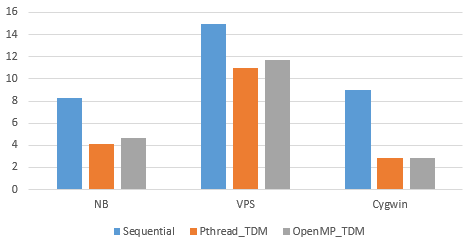
\includegraphics[width=\linewidth,natwidth=473,natheight=247]{white_platforms.png}
  \caption{White Balance (NB, VPS, Cygwin)}
  \label{fig:white_platforms}
\end{figure}

\subsection{White balance Profiling results}
When output is taken into account, the whole process is output-bound.
\begin{table}[H]
\centering
\begin{tabular}{|l|l|l|l|l|} \hline
Method&Total&Input&Calculate&Output\\ \hline
Sequential & 100\% & 29.41\% & 11.59\% & \textbf{59.00\%} \\ \hline
OpenMP & 100\% & 21.66\% & 7.29\% & \textbf{71.04\%} \\ \hline
\end{tabular}
\end{table}
\begin{figure}[H]
  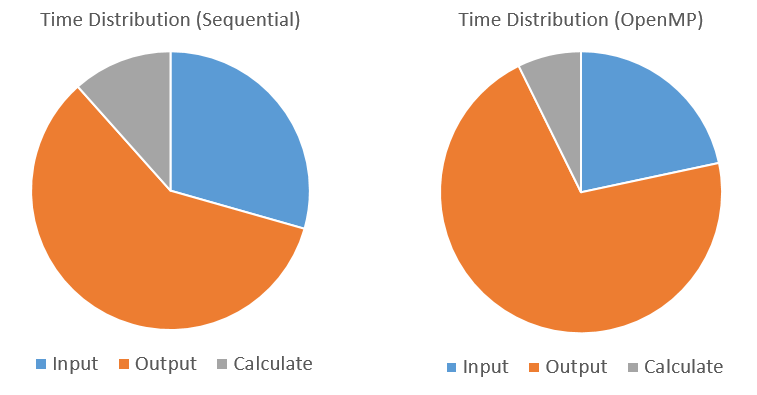
\includegraphics[width=\linewidth,natwidth=757,natheight=395]{profile.png}
  \caption{Profiling results (NB)}
  \label{fig:profile}
\end{figure}

\subsection{White balance when output is accounted}
Pthread\_with\_TaskParallel delivers better results(ie. higher efficiency) when output is taken in account.
\begin{figure}[H]
  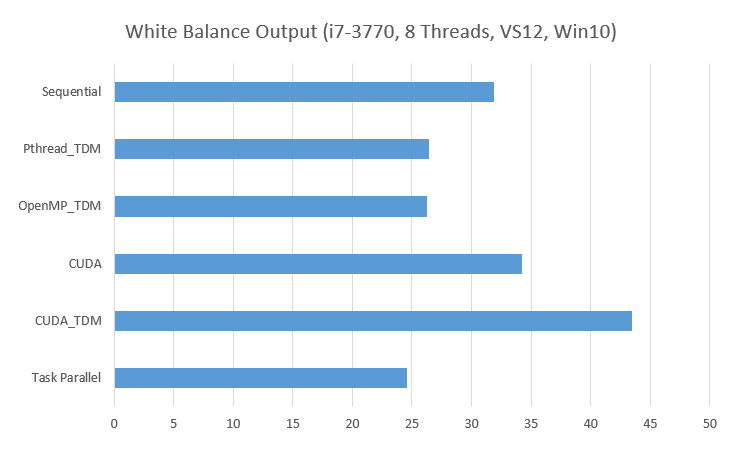
\includegraphics[width=\linewidth,natwidth=748,natheight=459]{taskparallel_pc.png}
  \caption{White balance with task parallel on main PC}
  \label{fig:taskparallel_pc}
\end{figure}
\begin{figure}[H]
  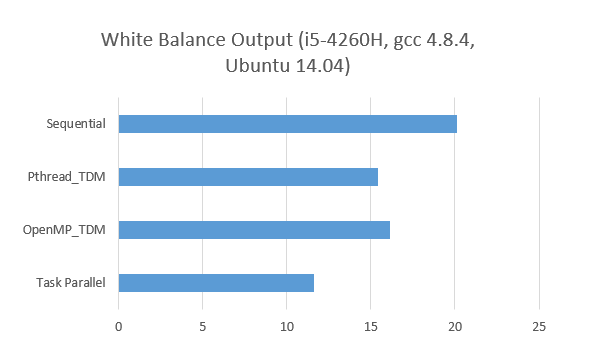
\includegraphics[width=\linewidth,natwidth=590,natheight=359]{taskparallel_nb.png}
  \caption{White balance with task parallel on NB}
  \label{fig:taskparallel_nb}
\end{figure}

\section{Related work}
\begin{itemize}
\item Ching-Chih Weng, Homer Chen, and Chiou-Shann Fuh. A Novel Automatic White Balance Method For Digital Still Cameras. In \textit{IEEE International Symposium on Circuits and Systems}, 2005.
\item Dennis Lin, Xiaohuang (Victor) Huang, Quang Nguyen, Joshua Blackburn, Christopher Rodrigues, Thomas Huang, Minh N. Do, Sanjay J. Patel, and Wen-Mei W. Hwu. The Parallelization of Video Processing. In \textit{IEEE Signal Processing Magazine}, pp. 103-112, November 2009.
\item Mihalis Psarakis, Aggelos Pikrakis, Giannis Dendrinos. FPGA-based Acceleration for Tracking Audio Effects in Movies. In \textit{IEEE 20th International Symposium on Field-Programmable Custom Computing Machines}, 2012.
\item Matthew Jacobsen, Yoav Freund, Ryan Kastner. RIFFA: A Reusable Integration Framework for FPGA Accelerators. In \textit{IEEE 20th International Symposium on Field-Programmable Custom Computing Machines}, 2012.
\end{itemize}

\section{Conclusions}
\begin{itemize}
\item Our experimental results show that certain hardware characteristics, memory bandwidth in particular, seem to be closely relevant to the efficiency of programs with linear complexities. We experienced a maximum 3.2x speedup on the Win10 desktop and a maximum 2x speedup on the Ubuntu laptop. Both were consistent with the pmbw test results from each of their platforms. It seems true that speedups do have upper bounds which depend on the hardware.
\item Additionally, we think we should keep simple computations on the CPU end. Using NVIDIA's Nsight profiling tool, we were able to identify huge memory bottlenecks over the course of the program execution. It is perhaps futile to parallelize simple linear-complexity algorithms as the time it takes to copy the data between host and device would be relatively significant. Things could be better on a workstation-grade GPU though.
\item Moreover, it seems that FPGAs handle parallel programming extremely well. Past research has  shown that using FPGAs as accelerators can realize better performance than using GPGPUs. It does hold true in our experiments. In our opinion, it's probably safe to say that FPGAs are great tools for applications demanding massive computations.
\item Lastly, the video codec used for input also seems to matter. When the input video is encoded in mp4 format, parallelizing the input procedure actually slows down the whole process. It took us quite a bit of effort to accomplish the results we have right now. A reasonable guess for this would be, perhaps non-sequential reads caused slight delays in between and longer decoding times potentially triggered unwanted queueing effects.
\end{itemize}

\section{Endnotes}
\begin{itemize}
\item We would like to thank Prof. Yi-Ping You, Assistant Professor at the Department of Computer Science, National Chiao Tung University and the teaching assistants for an excellent course (Parallel Programming, Fall 2015). The knowledge we gained throughout the course helped us tremendously.
\item We would also like to thank Prof. Chun-Jen Tsai, Associate Professor at the Department of Computer Science, National Chiao Tung University for lending the FPGA board (ML506 Evaluation Platform) to us and for all the advices he offered during the research.
\item Collaborated project. All sources are publicly available on GitHub: \\
\url{https://github.com/sunset1995/parallel_analysis} \\
\url{https://github.com/yuwen41200/fpga-computing}
\end{itemize}

\begin{thebibliography}{9}
\bibitem{pmbw}
Timo Bingmann. (2013).
pmbw - Parallel Memory Bandwidth Benchmark / Measurement.
Available at \url{http://panthema.net/2013/pmbw/}

\bibitem{gray_world} 
Jason Su. (2010).
Illuminant Estimation: Gray World. 
Available at \url{http://web.stanford.edu/~sujason/ColorBalancing/grayworld.html}

\bibitem{fpga_ref} 
Xillybus Ltd. (2016).
An FPGA IP Core for Easy DMA over PCIe with Windows and Linux [Online]. 
Available at \url{http://xillybus.com/.}
\end{thebibliography}

\end{document}
